\documentclass{article}
\usepackage[utf8]{inputenc}
\usepackage{graphicx}

\title{Relatório - Introdução à Computação Científica}
\author{Henrique Luiz Rieger e Leon Augusto Okida Gonçalves}
\date{Dezembro de 2021}

\begin{document}

\maketitle

\newpage
\section{Introdução}
Este trabalho foi feito para a disciplina de Introdução à Computação Científica, ministrada pelos professores Armando Luiz Nicolini Delgado e Guilherme Alex Derenievicz.\\
Ele consiste em otimizações feitas em cima do código do primeiro trabalho da disciplina e em um experimento, onde comparamos os desempenhos das duas versões.\\
Neste texto, relataremos as melhorias feitas e exibiremos os resultados do experimento.

\newpage
\section{Máquina usada nos experimentos}
A CPU da máquina usada nos experimentos é um Intel i7-7000 Coffeelake, com frequência de 3.60GH.\\
Ela conta com 1 socket, 4 cores por socket e 2 threads por core, sendo um total de 8 threads.\\
Tem 3 níveis de cache, com L1 com espaço de 32 kB, L2 com 256 kB e L3 com 8 MB.\\
A máquina tem também 16 GB de memória RAM.

\newpage
\section{Como executar os experimentos}
Para executar os experimentos, basta executar \texttt{./script.sh} no diretório principal do trabalho.\\
Após isso, deve-se inserir a senha do usuário, o que fará com que os experimentos sejam iniciados.\\
Por fim, deve-se aguardar o término dos experimentos. Os gráficos e resultados serão gerados automaticamente.

\newpage
\section{Alteração feita na contagem de tempo}
Foi feita uma mudança na contagem de tempo do cálculo das derivadas parciais, para desconsiderar o tempo gasto com a alocação dinâmica da matriz.\\
Essa alteração foi feita tanto no código antigo bem como no código otimizado.

\newpage
\section{Otimizações feitas}
Foram feitas as seguintes otimizações:

\subsection{Estrutura da matriz de derivadas parciais}
No trabalho 1, ela era estruturada como um vetor de ponteiros de linhas separadas. Isso foi mudado, sendo agora um vetor único, com os acessos sendo feitos por meio de aritmética de ponteiros.\\
Isso favorece o acesso rápido à memória, pois seus elementos estão em posições contíguas, tendo uma boa localidade de referência.\\
É importante notar que o tipo da matriz mudou de \texttt{void***} para \texttt{void**}.\\
Essa otimização exigiu também a mudança de diversas partes do código, tanto em argumentos de funções bem como no acesso à matriz.\\
A estrutura da matriz está em \texttt{vetoresOpt.c}.

\subsection{Considerando a tridiagonalidade}
Foram feitas mudanças na função de alocação e cálculo da matriz de derivadas parciais, para refletir a triagonalidade dela.\\
Os cálculos da primeira linha e da última linha foram feitos fora do laço, que engloba apenas as linhas intermediárias.\\
Isso reduz o número de operações feitas.\\
Isso é feito no arquivo \texttt{vetoresOpt.c}.

\subsection{Padding}
Foi feito padding em vetores/matrizes de tamanho da forma $2^k$, a fim de evitar cache misses.\\
Isso foi implementado com uma macro em \texttt{utils.h}.

\subsection{Restrict Pointers}
Foram usados restrict pointers, que fazem com que o processador entenda que não há dependências implícitas, permitindo que ele faça otimizações adicionais.

\subsection{Inversão no cálculo de F(X)}
Durante o cálculo de F(X), a inversão é feita inline, para evitar alterações desnecessárias depois.\\
Isso é feito no arquivo \texttt{newtonOpt.c}.

\subsection{Valores abaixo da diagonal principal}
Os valores que estão abaixo da diagonal principal não são zerados, pois são desnecessários para cálculos com matrizes tridiagonais.\\
Isso poupa acessos à memória.

\subsection{Valores na Jacobiana}
Os valores da Matriz Jacobiana são salvos em variáveis durante os cálculos, para evitar FLOPS desnecessários.

\newpage
\section{Gráficos gerados}
\subsection{Cálculo das derivadas parciais}

\begin{figure}[htp]
    \centering
    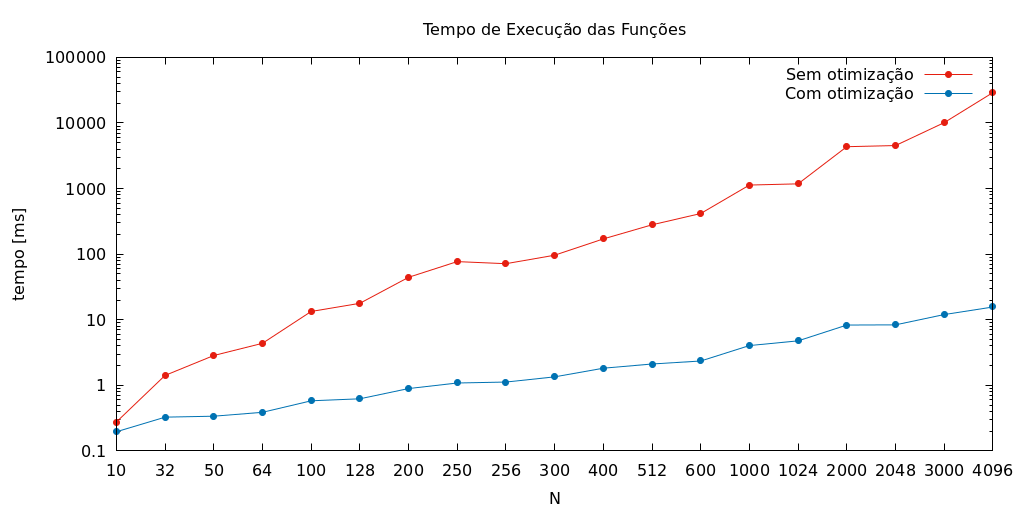
\includegraphics[width=12cm]{tempo_derivadas.png}
    \caption{Gráfico do tempo do cálculo da matriz de derivadas parciais}
    \label{fig:tempo_derivadas}
\end{figure}

\begin{figure}[htp]
    \centering
    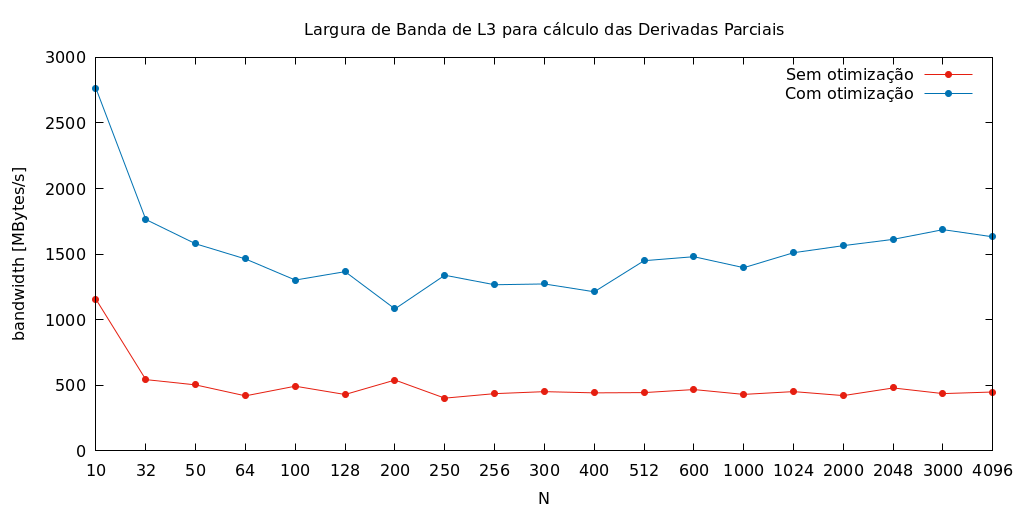
\includegraphics[width=12cm]{l3_derivadas.png}
    \caption{Gráfico da banda de memória do cálculo da matriz de derivadas parciais}
    \label{fig:l3_derivadas}
\end{figure}

\begin{figure}[htp]
    \centering
    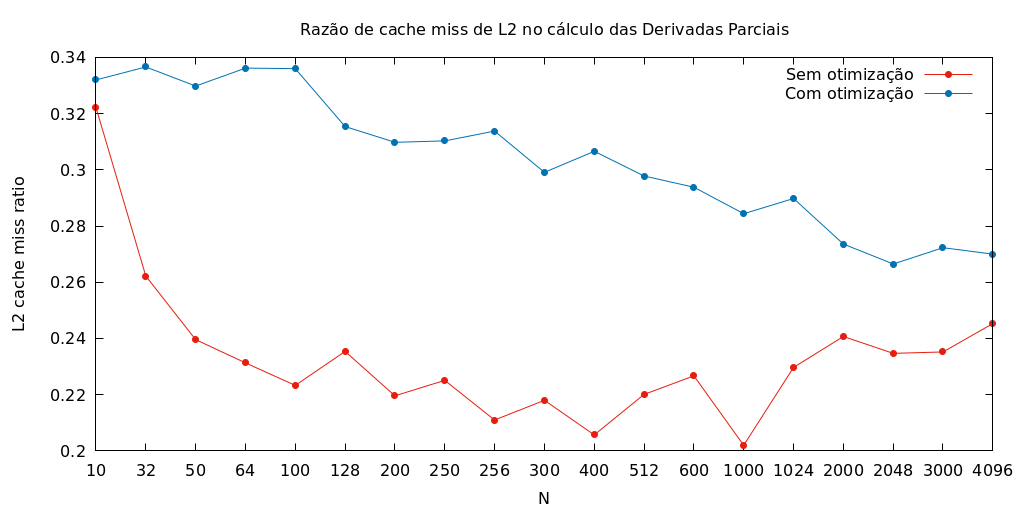
\includegraphics[width=12cm]{l2cache_derivadas.png}
    \caption{Gráfico de cache misses do cálculo da matriz de derivadas parciais}
    \label{fig:l2_derivadas}
\end{figure}

\begin{figure}[htp]
    \centering
    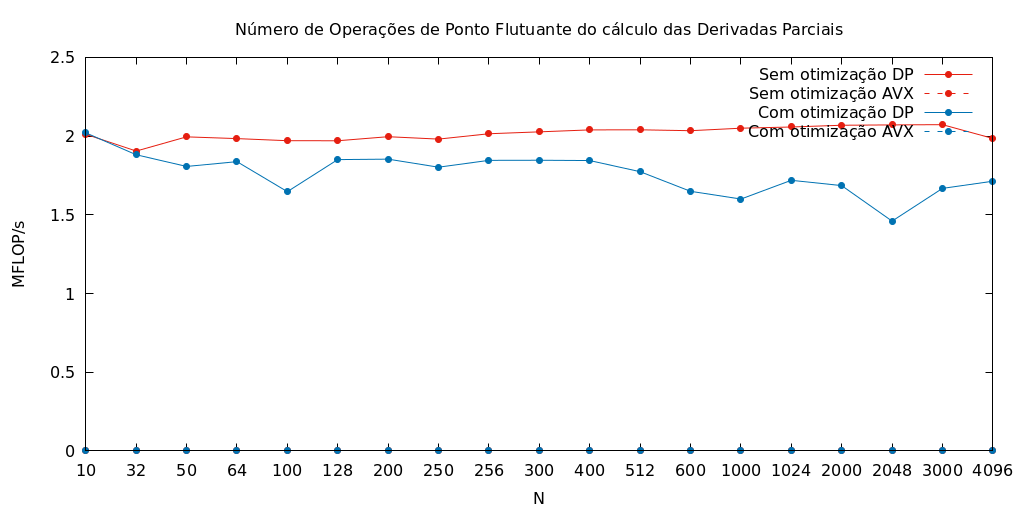
\includegraphics[width=12cm]{flops_dp_derivadas.png}
    \caption{Gráfico de operações de ponto flutuante do cálculo da matriz de derivadas parciais}
    \label{fig:flops_derivadas}
\end{figure}

\newpage
\subsection{Método de Newton}

\begin{figure}[htp]
    \centering
    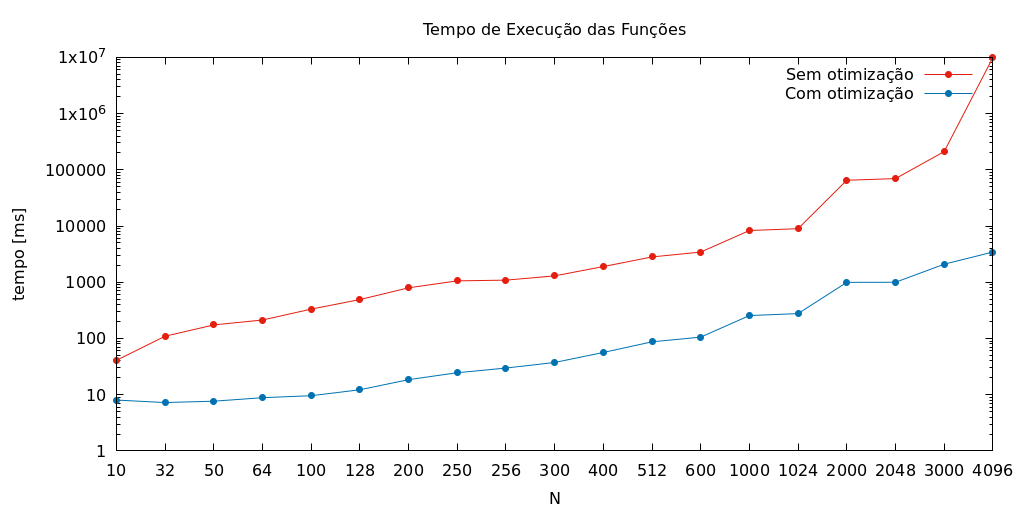
\includegraphics[width=12cm]{tempo_newton.png}
    \caption{Gráfico do tempo do método de Newton}
    \label{fig:tempo_newton}
\end{figure}

\begin{figure}[htp]
    \centering
    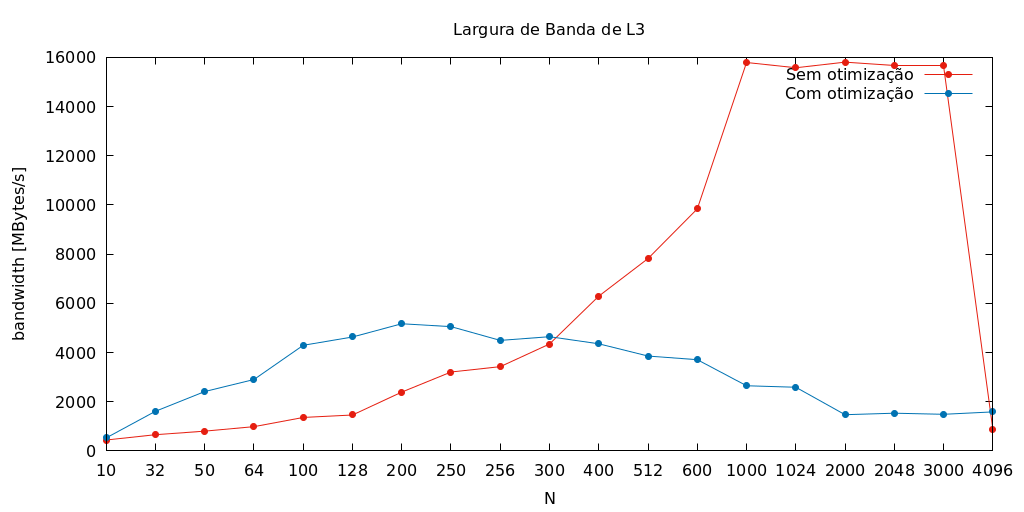
\includegraphics[width=12cm]{l3_newton.png}
    \caption{Gráfico da banda de memória do método de Newton}
    \label{fig:l3_newton}
\end{figure}

\begin{figure}[htp]
    \centering
    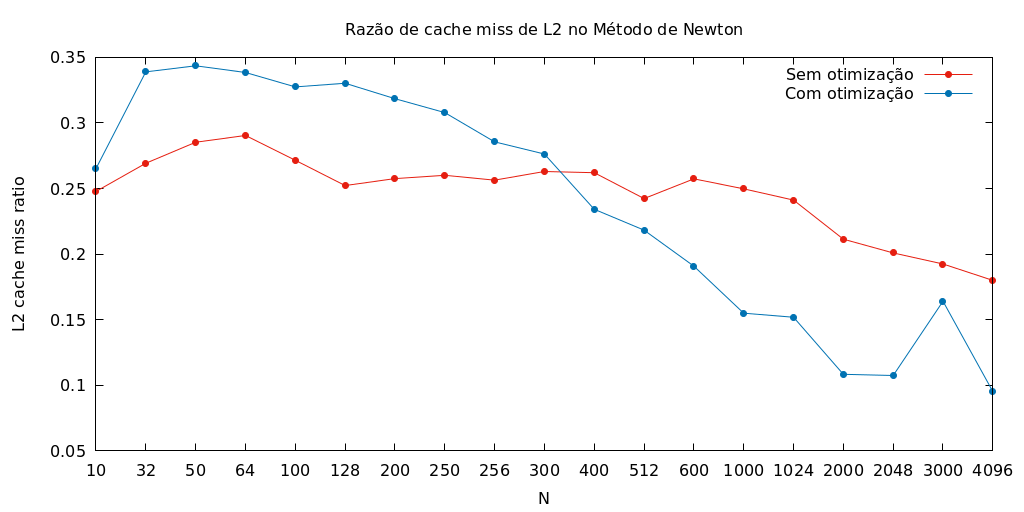
\includegraphics[width=12cm]{l2cache_newton.png}
    \caption{Gráfico de cache misses do método de Newton}
    \label{fig:l2_newton}
\end{figure}

\begin{figure}[htp]
    \centering
    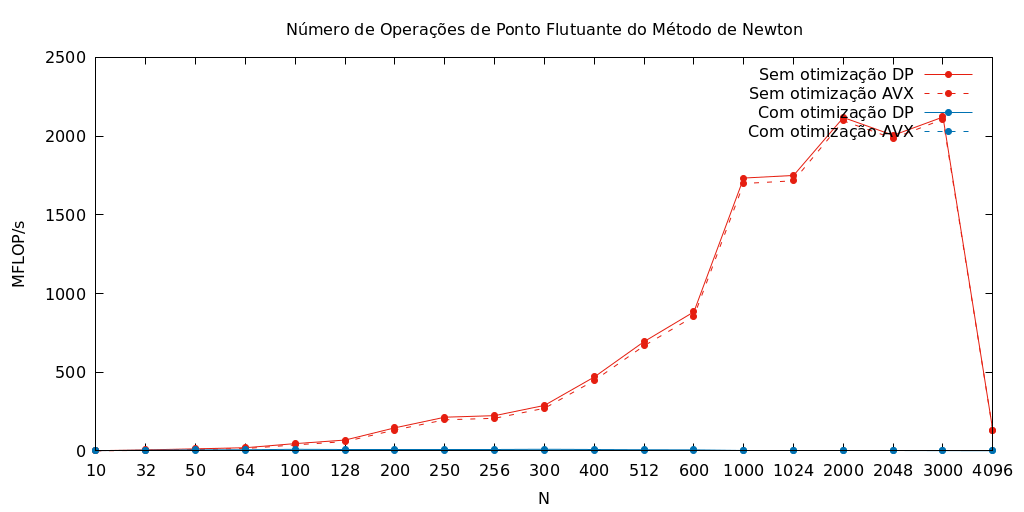
\includegraphics[width=12cm]{flops_dp_newton.png}
    \caption{Gráfico de operações de ponto flutuante do método de Newton}
    \label{fig:flops_newton}
\end{figure}

\newpage
\subsection{Cálculo das Matrizes Jacobianas}

\begin{figure}[htp]
    \centering
    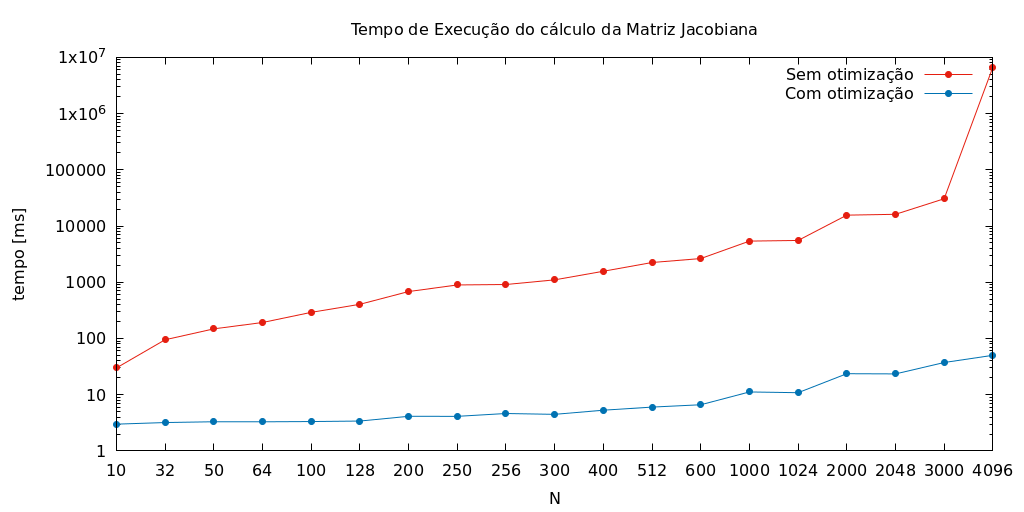
\includegraphics[width=12cm]{tempo_jacobiana.png}
    \caption{Gráfico do tempo do cálculo das Matrizes Jacobianas}
    \label{fig:tempo_jac}
\end{figure}

\begin{figure}[htp]
    \centering
    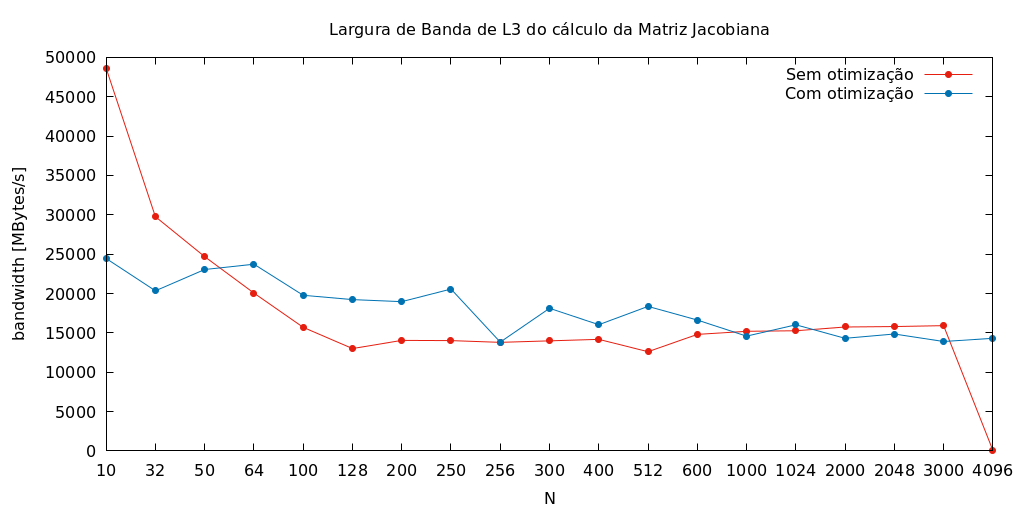
\includegraphics[width=12cm]{l3_jacobiana.png}
    \caption{Gráfico da banda de memória do cálculo das Matrizes Jacobianas}
    \label{fig:l3_jac}
\end{figure}

\begin{figure}[htp]
    \centering
    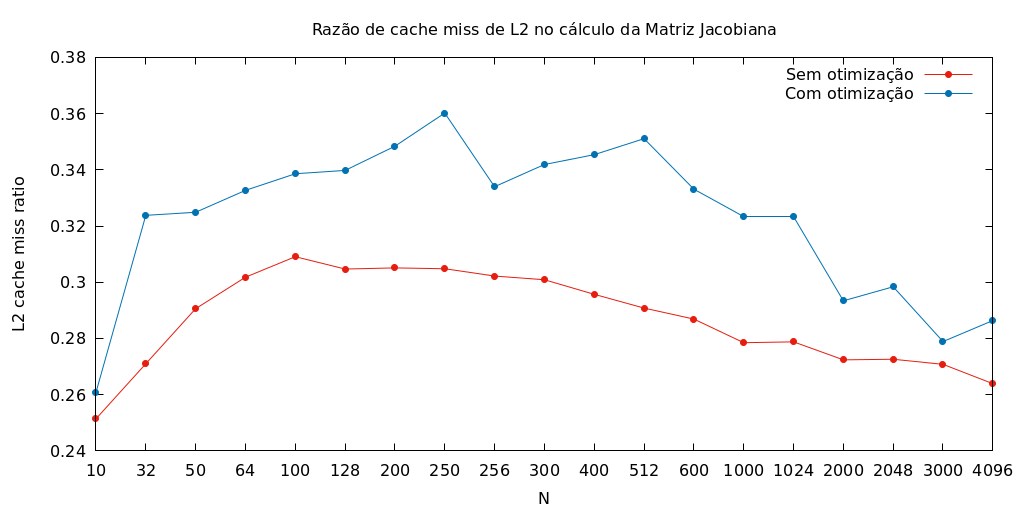
\includegraphics[width=12cm]{l2cache_jacobiana.png}
    \caption{Gráfico de cache misses do cálculo das Matrizes Jacobianas}
    \label{fig:l2_jac}
\end{figure}

\begin{figure}[htp]
    \centering
    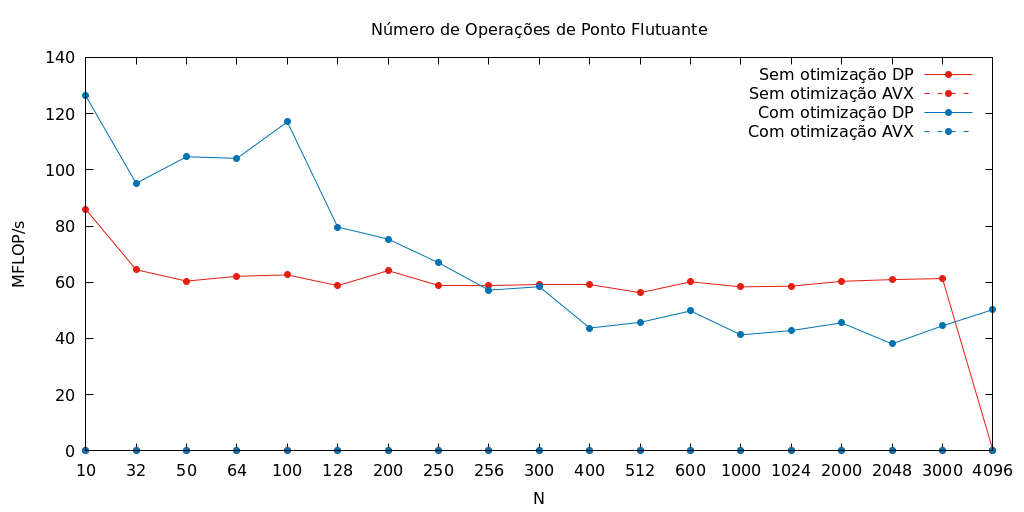
\includegraphics[width=12cm]{flops_dp_jacobiana.png}
    \caption{Gráfico de operações de ponto flutuante do cálculo das Matrizes Jacobianas}
    \label{fig:flops_jac}
\end{figure}

\newpage
\subsection{Resolução dos Sistemas Lineares}

\begin{figure}[htp]
    \centering
    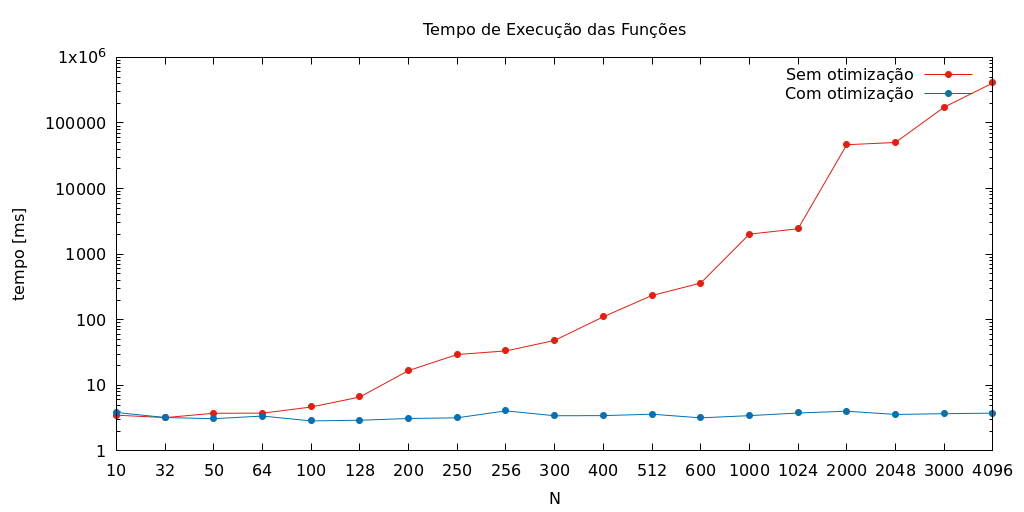
\includegraphics[width=12cm]{tempo_sistema_linear.png}
    \caption{Gráfico do tempo da resolução dos Sistemas Lineares}
    \label{fig:tempo_sl}
\end{figure}

\begin{figure}[htp]
    \centering
    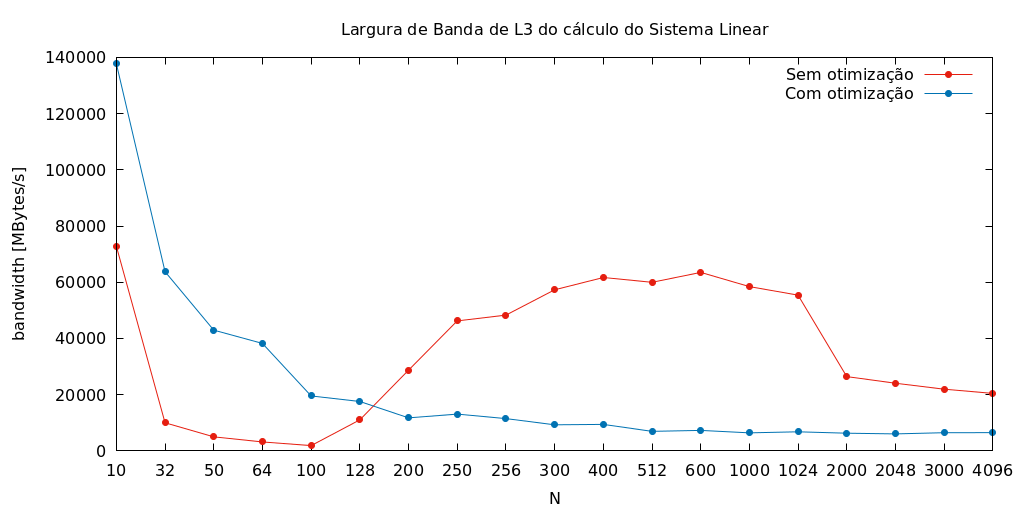
\includegraphics[width=12cm]{l3_sistema_linear.png}
    \caption{Gráfico da banda de memória da resolução dos Sistemas Lineares}
    \label{fig:l3_sl}
\end{figure}

\begin{figure}[htp]
    \centering
    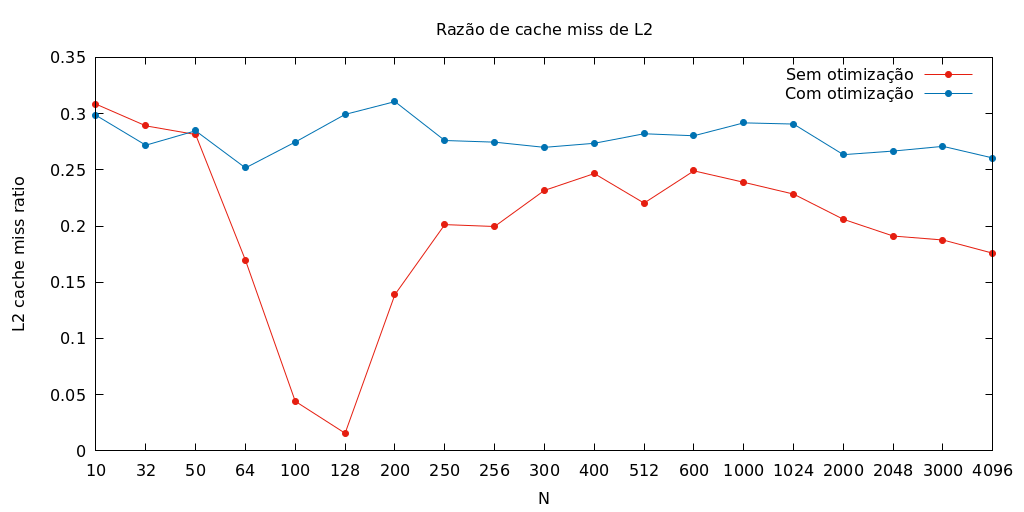
\includegraphics[width=12cm]{l2cache_sistema_linear.png}
    \caption{Gráfico de cache misses da resolução dos Sistemas Lineares}
    \label{fig:l2_sl}
\end{figure}

\begin{figure}[htp]
    \centering
    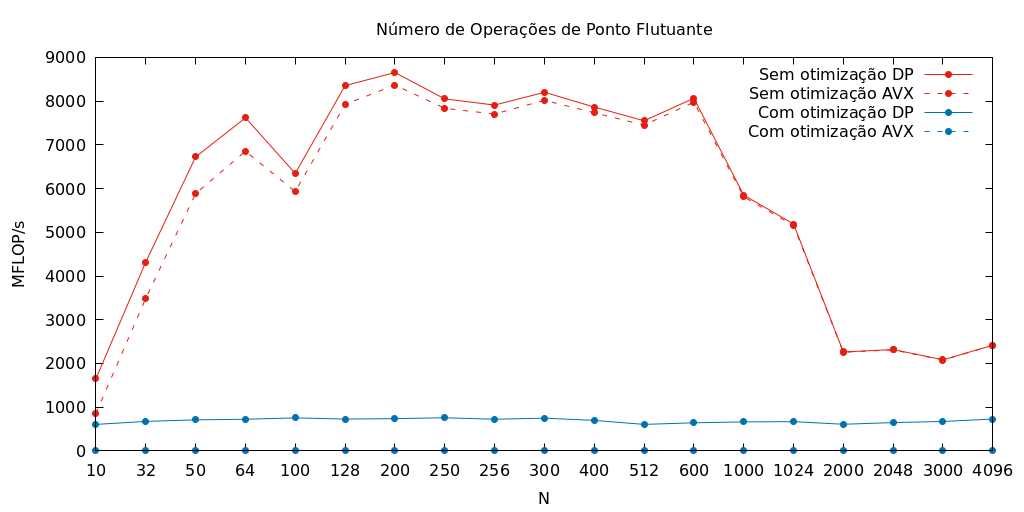
\includegraphics[width=12cm]{flops_dp_sistema_linear.png}
    \caption{Gráfico de operações de ponto flutuante da resolução dos Sistemas Lineares}
    \label{fig:flops_sl}
\end{figure}

\end{document}
